\documentclass[12pt]{article}

\usepackage{sbc-template}

\usepackage{graphicx,url}

\usepackage[brazil]{babel}   
%\usepackage[latin1]{inputenc}  
\usepackage[utf8]{inputenc}  
% UTF-8 encoding is recommended by ShareLaTex

\usepackage{mdframed}
\usepackage{minted}
\usepackage{hyperref}
\usepackage{amssymb}
     
\sloppy

\title{Trabalho Prático 3 - Redes Neurais Artificiais}

\author{Hugo Araujo de Sousa}

\address{
  Computação Natural (2017/2) \\
  Departamento de Ciência da Computação \\
  Universidade Federal de Minas Gerais (UFMG)
  \email{hugosousa@dcc.ufmg.br}
}

\begin{document} 

\maketitle
     
\begin{resumo}
  Nesse trabalho são explorados conceitos relacionados a redes neurais,
  colocando-os em prática através da utilização da biblioteca Keras com Tensorflow, 
  que nos permite abordar um problema de classificação.
\end{resumo}

\section{INTRODUÇÃO}

Dentro da área de Computação Natural, o campo de Redes Neurais Artificiais
tem como objetivo a criação de modelos computacionais inspirados pelo
conhecimento que temos sobre como funciona o sistema nervoso, mais
especificamente, na estrutura e função dos neurônios no cérebro
\cite{clevalg}.

Dessa forma, uma Rede Neural Artificial é uma coleção de neurônios
artificiais que são conectados a fim de se realizar alguma computação
em padrões de entrada para gerar padrões de saída. Esses neurônios,
então, se adaptam, modificando sua estrutura interna ao longo do tempo.
Geralmente, essa modificação se dá através da atualização dos pesos
das conexões entre os neurônios da rede. Esse processo define o
aprendizado da rede neural, que então se torna, com o tempo, cada
vez mais adaptada na tarefa de gerar o padrão de saída correto de 
acordo com a entrada.

No trabalho em questão, usaremos a biblioteca Keras 
\footnote{\url{https://keras.io/}} com Tensorflow
\footnote{\url{https://www.tensorflow.org/}}, que juntas fornecem
implementações de redes neurais já prontas para uso. A partir dessas 
duas bibliotecas, o problema a ser resolvido será o de classificação
de um conjunto de dados específico.

Esse conjunto de dados reúne informações de 1429 proteínas, descritas
por 8 atributos (números reais). Para cada uma dessas proteínas, a sua
classe se refere à parte da célula em que a proteína se encontra.
Ao todo, existem 7 classes possíveis, descritas na Tabela
\ref{tab:classes}.

\begin{table}[h]
	\centering
	\begin{tabular}{|c|c|}
		\hline
		\textbf{Classe} & \textbf{Descrição} \\ \hline
		\textbf{CYT} & Citoplasma \\ \hline
		\textbf{MIT} & Mitocôndria \\ \hline
		\textbf{ME1} & Uma membrana específica da célula \\ \hline
		\textbf{ME2} & Uma membrana específica da célula \\ \hline
		\textbf{ME3} & Uma membrana específica da célula \\ \hline
		\textbf{EXC} & Exterior da célula \\ \hline
		\textbf{NUC} & Núcleo da célula \\ \hline
	\end{tabular}
	\caption{\label{tab:classes} Classes que descrevem a posição
	das proteínas em uma célula.}
\end{table}

Portanto, a rede neural criada será alimentada com os dados dessa base e,
ao longo do tempo, tentará aprender os padrões que determinam a saída
da mesma, isto é, dado um conjunto de 8 atributos de uma proteína, a
rede deve dizer qual é a posição que essa proteína ocupa na célula (
representada pela classe, dentre as 7 descritas acima).

\section{MODELAGEM}

Para modelar esse problema, o primeiro passo é determinar qual o tipo
da rede neural a ser construída - existem vários tipos de arquitetura
de redes neurais diferentes.

Para o trabalho em questão, optou-se por simplicidade em termos de
representação, o que, por sua vez, acarreta em maior controle sobre 
a estrutura da rede e de seu funcionamento. Dessa forma, a arquitetura
escolhida foi a \textit{Multilayer Perceptron - MLP} (Perceptron de
múltiplas camadas), que é uma versão da rede \textit{Perceptron} 
generalizada para conter múltiplas camadas escondidas de neurônios.
A Figura \ref{fig:mlp} mostra a estrutura da rede MLP.

\begin{figure}[!htbp]
  \centering
  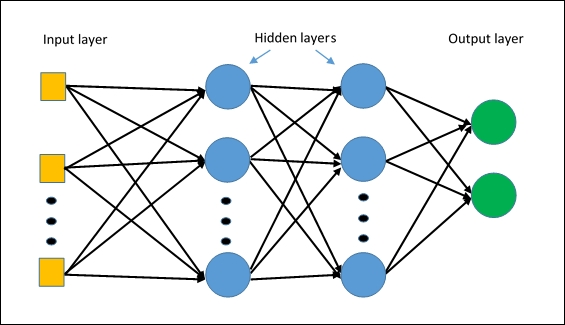
\includegraphics[width=1\textwidth]{mlp.jpg}
  \caption{Estrutura da rede \textit{Multilayer Perceptron}. Vemos
  que, além das camadas de entrada e saída, a rede também pode
  apresentar um número arbitrário de camadas escondidas de neurÕnios.
  O número de neurônios em cada camada também pode ser escolhido
  arbitrariamente.}
  \label{fig:mlp}
\end{figure}

\section{IMPLEMENTAÇÃO}



\section{ESTRUTURA DO PROJETO E EXECUÇÃO}



\section{EXPERIMENTOS}



\section{CONCLUSÃO}



\section{REFERÊNCIAS}



\bibliographystyle{sbc}
\bibliography{sbc-template}

\end{document}
